This test case is identical to Case~1a described above, except for the use of the Beta distribution for the vulnerability functions instead of the lognormal distribution. Since the coefficients of variation in the vulnerability function are all zero, once again the Beta distribution devolves into the degenerate distribution as in Case~1a. The results for this test case should be exactly the same as in Case~1a.

The loss curve calculated using the implementation of the calculator in Julia is compared with that produced by OpenQuake in Figure~\ref{fig:lc-ebr-1e}.

\begin{figure}[htbp]
\centering
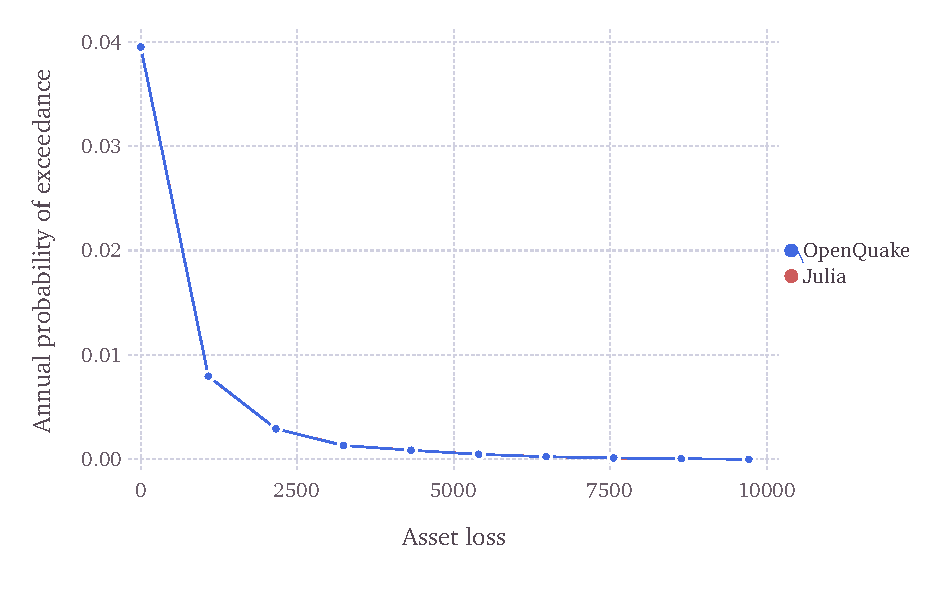
\includegraphics[width=12cm]{qareport/figures/fig-lc-ebr-1e}
\caption{Loss curve comparison for event based risk test case 1e}
\label{fig:lc-ebr-1e}
\end{figure}

The area under the annual loss exceedance curve gives the average annual loss.